\section{Initial Approach - Classification}
Here we report our initial experiments where we formulated the task of predicting near-collision time as a classification model. 

\subsection{Binary Classification: What happens 1 second into the future?}

In initial experimentation, we formulated the task as binary classification whether there is a near-collision in next one second or not. The output layer in Fig. \ref{fig:model} is replaced by a two-neuron layer followed by softmax function. The binary cross entropy loss is used to train the network. An alternative naive way to solve this task is to compare the foot of pedestrians' bounding boxes with a predefined threshold on pixel's vertical coordinate. The table \ref{tab:binary_classification} compares the F1 score from our learning approach versus the naive baseline. For the naive baseline, if the foot of the pedestrian lies in the lower $37.5\%$ (empirically found to be best) of the vertical size of image, we classify it as collision within one second.  \\

We use GradCAM \cite{gradCAM} to see which part of the image our trained network attends to. 
\begin{align*}
    {\alpha_k}^{c} = \frac{1}{Z}\sum_{i}\sum_{j}\frac{\delta y^{c}}{\delta {A_{ij}}^{k}} \\
    L^{c} = ReLU(\sum_{k} \alpha_{k}^{c}A_{k})\\
    y_c: \text{Score for the class $c$}\\
    {\alpha_k}^{c}: \text{Weight for $k^{th}$ channel in last convolutional map for class $c$}\\
    A_{ij}^{k}: \text{Activation of $(i, j)$ in $k^{th}$ convolutional channel}\\
    L^{c}: \text{Heatmap for class $c$}
\end{align*}
It first computes the gradient of the score for a class $c$ with respect to the activations of last convolutional layer. The gradients are global-average-pooled to get the importance of a feature map $k$ for class $c$, denoted as ${\alpha_k}^{c}$. A weighted combination of forward activation maps is finally upsampled to the  size of input image to visualize the attention map. The confusion matrix over a test set passed through the trained network is reported in table \ref{tab:confusion_matrix}. To tackle the data imbalance between the collision instances (2106) and no collision instances (8579), a weighted sampler is used in training with collision instances having a weight of $0.6$ and no collision instances having a lower weight of $0.4$.
%% I should balance the training! 

    \begin{figure}[ht]
      \centering
      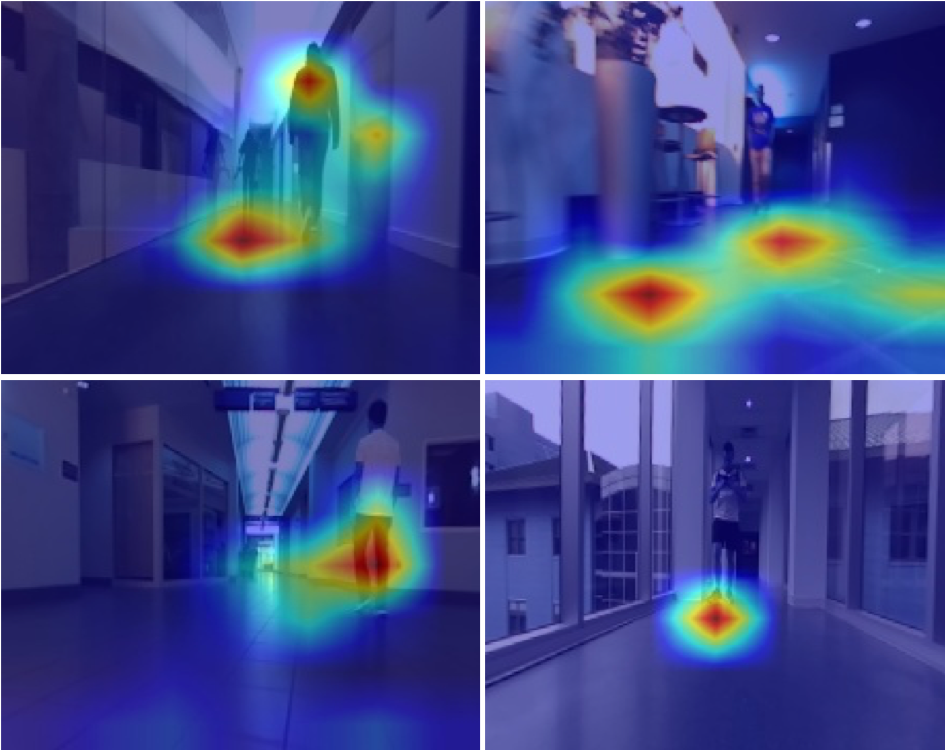
\includegraphics[height=8cm, width=\columnwidth]{figs/grad_binary_class.png}
      \caption{Visualization of attention maps using GradCAM; Top Left: Two Persons going away, Top Right: One person with two probable trajectories, Bottom Left: A person going away, Bottom Right: A person approaching}
      \label{fig:gradcam1}
  \end{figure}

    \begin{figure}[ht]
      \centering
      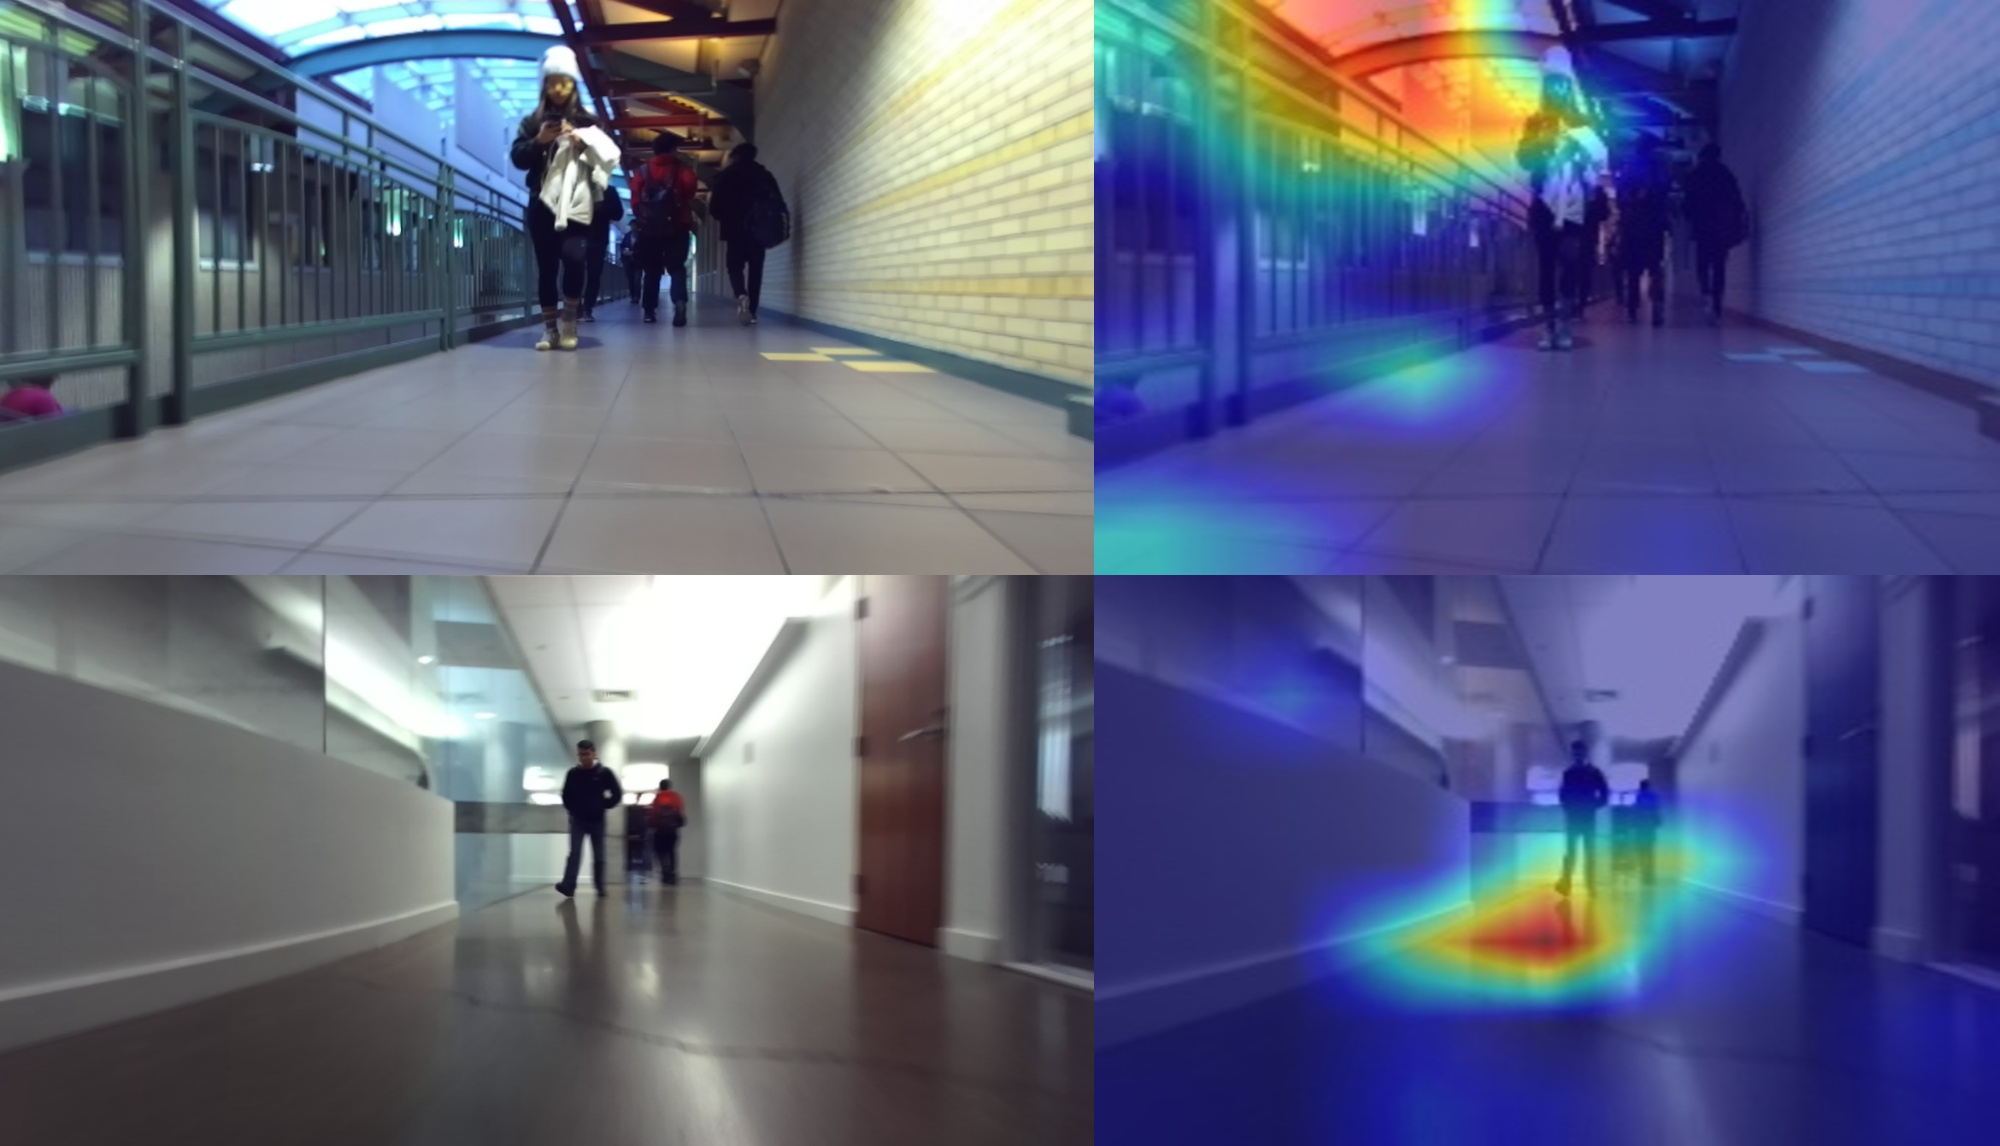
\includegraphics[height=8cm, width=\columnwidth]{figs/gradCAM.pdf}
      \caption{Left: RGB Image, Right: Corresponding GradCAM}
      \label{fig:gradcam2}
  \end{figure}

\begin{table}[h]
\caption{Confusion Matrix from Binary Classification}\label{tab:confusion_matrix}
\noindent
\renewcommand\arraystretch{1.5}
\setlength\tabcolsep{0pt}
\begin{tabular}{c >{\bfseries}r @{\hspace{0.7em}}c @{\hspace{0.4em}}c @{\hspace{0.7em}}l}
  \multirow{10}{*}{\parbox{1.1cm}{\bfseries\raggedleft Actual\\ value}} & 
    & \multicolumn{2}{c}{\bfseries Prediction outcome} & \\
  & & \bfseries \small{collision} & \bfseries \small{no collision} \\
  & \small{collision} & \MyBox{634}{} & \MyBox{36}{} \\[2.4em]
  & \small{no collision} & \MyBox{53}{} & \MyBox{2840}{}  
\end{tabular}
\end{table}

\begin{table}[h]
\caption {Near-Collision Prediction formulated as Binary Classification: F1 Scores from our approach compared with a naive baseline} \label{tab:binary_classification} 
\begin{tabular}{|P{4cm}|P{2cm}|} \hline
Method  &  F1 Score \\ \hline
Naive baseline $(0.625 Y)$ & 0.8488 \\ \hline 
N-stream VGG $(N = 4)$ &  \textbf{0.9344} \\ \hline %% From slides  
\end{tabular}
\end{table}

\subsection{Multi-label Classification}
On previous task of binary classification for 0-1 sec, our deep learning approach performs better than the naive thresholding as reported in table \ref{tab:binary_classification}. We thus move on to increasing the difficulty of the task, i.e, a multi-label classification problem where we classify if there is going to be a near-collision instance in (1) within a second, (2) between 1-2 seconds, (2) between 2-3 seconds and/or (4) after 3 seconds. Our training and test data distribution for this multi-label classfication is provided in table \ref{tab:class_distribution}. For training, we used multilabel soft margin loss \cite{pytorch} as the loss function. The F1 scores reported in table \ref{tab:multi_label_classification} indicates that the naive baseline can give better predictions within 2 seconds into the future while the proposed multilabel deep neural network performs better for the latter classes, i.e., predictions in the range 2-3 seconds and after 3 seconds. One of the challenges of this multi-label formulation over the regression formulation is that we have to empirically decide a threshold on the confidence score for each class to classify it as the positive or negative label. The precision-recall curve or area under ROC curve \cite{roc} can be used to evaluate the performance of the trained model at different thresholds and then decide a threshold accordingly. \\

\begin{table}[h]
\caption {Class Distribution} \label{tab:class_distribution} 
\begin{tabular}{|P{4cm}|P{4cm}|P{4cm}|} \hline
Near-Collision Time  &  Training Data & Test Data \\ \hline
0-1 s &  4150 & 287 \\ \hline 
1-2 s &  2590 & 185 \\ \hline
2-3 s &  2185 & 169 \\ \hline
After 3 s & 13049  & 507 \\ \hline 
\end{tabular}
\end{table}

\begin{table}[h]
\caption {Near-Collision Prediction formulated as Multi-Class Classification} \label{tab:multi_label_classification} 
\begin{tabular}{|P{4cm}|P{4cm}|P{3cm}|P{3cm}|} \hline
Near-Collision Time  &  Vertical Image Coordinate for naive baseline $Y = 720$  & F1 Score from Naive Baseline & F1 Score from N-Stream VGG \\ \hline
0-1 s & $> 0.625Y$ &  0.849 & 0.759 \\ \hline 
1-2 s & $> 0.560Y$ & 0.720 & 0.630 \\ \hline
2-3 s & $> 0.520Y$ & \textbf{0.629} & \textbf{0.947} \\ \hline
After 3 s & $\le 0.520Y$ & \textbf{0.522}  & \textbf{0.620} \\ \hline 
\end{tabular}
\end{table}
 
 
  \begin{figure*}[ht]
      \centering
      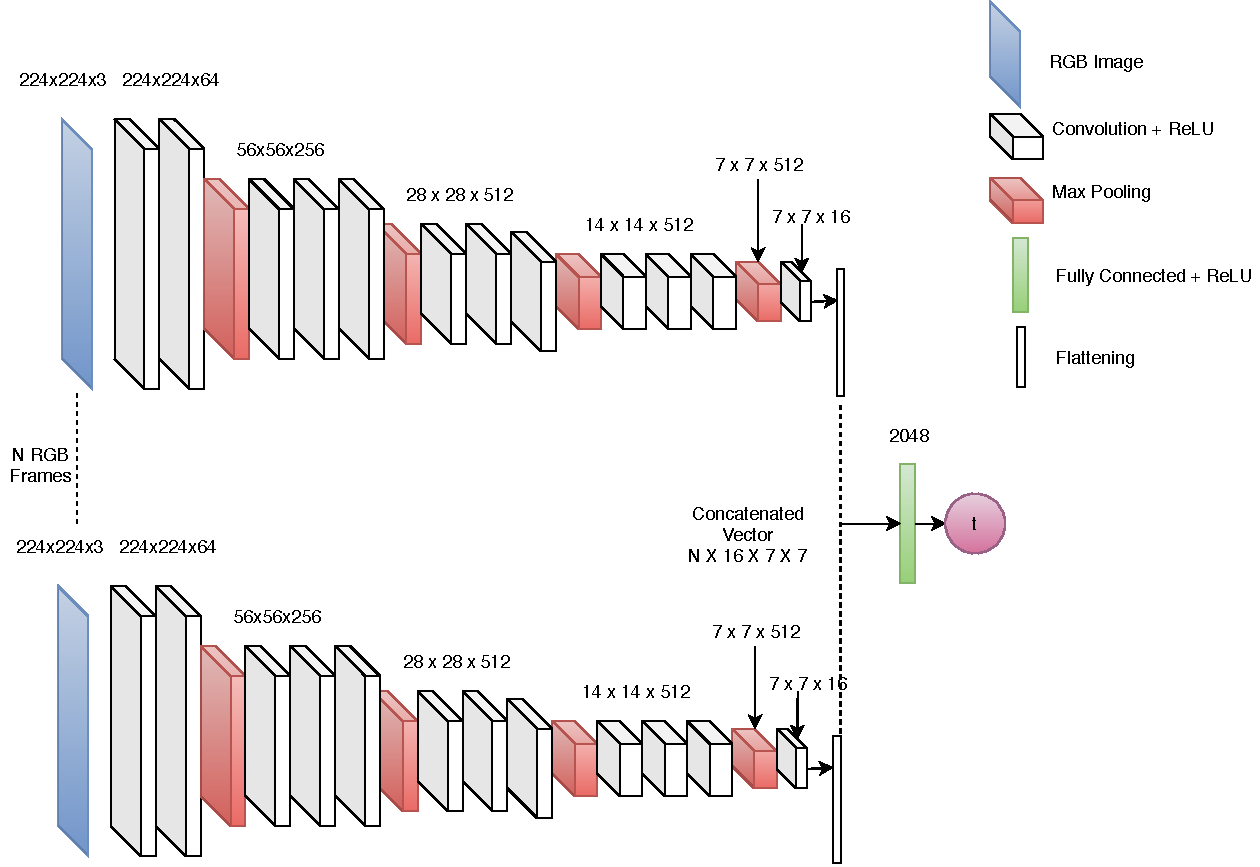
\includegraphics[height=7.0cm, width=12cm]{figs/vgg_2.pdf}
      \caption{Our model with VGG-16 as backbone where the final output is time to collision denoted as $t$ }
      \label{fig:model}
  \end{figure*}

Our goal is to predict the time at which at least one person is going to come within a meter distance of the mobile setup using only a monocular image sequence of $N$ frames. The video is recorded at $10$ fps and thus a sequence of $N$ frames, including the current frame and past $(N-1)$ frames, correspond to the history of $\frac{N-1}{10}$ seconds. We first provide a formal definition of the task and then the details of network architecture for reproducibility.   

\section{Problem Formulation - Classification or Regression?}

Learning time to near-collision can be formulated as a multi-class classification into one of the 60 classes where $i^{th}$ class corresponds to time range between $(\frac{i-1}{10}, \frac{i}{10}]$ seconds. The disadvantage of training it as a classification task is that all the mispredictions are penalized equally. For example, let us consider two different mispredictions given the same ground truth of 0.5 seconds - one where the network categorized it into the class $(0.6, 0.7]$ and other when the network predicted $(5.5, 5.6]$. The multi-class cross-entropy loss on both of these will be equal while we want the latter to be penalized much more than the former. One of the solutions is to design a differentiable loss function which keeps this preference in mind. Another solution is to formulate it as a regression problem and use the mean-squared error as the loss function. In this paper, we formulated it as a regression problem as follows:
$$
%t = f(image_{1}, image_{2}, \hdots, image_{N}) \text{ where } t \in [0, 6]
t = f(I_{1}, I_{2}, \hdots, I_{N}) \text{ where } t \in [0,6]
$$

\section{Network Architecture}
%% Why I chose VGG-16?
%% ImageNet do not have a person class, thus the network was fine-tuned on PASCAL VOC dataset 
%% We propose a N-stream network where each stream takes in the $i^{th}$ image  
VGG-16 \cite{vgg} is a 16-layer convolutional neural network which won the localization task in ImageNet Challenge 2014. It used parameter efficient $3 \times 3$ convolutional kernels pushing the depth to 16 weight layers. It was shown that its representations generalize well to other datasets achieving state-of-the-art results. We propose a multi-stream VGG architecture as shown in Fig. \ref{fig:model} where each stream takes a $224 \times 224$ RGB frame as input to extract spatial features . These spatial features are then concatenated across all frames preserving the temporal order and then fed into a perceptron to output time to collision. \\

% The inputs to the network are short N-frame clips corresponding to a temporal footprint of $\frac{N-1}{10}$ seconds. The concatenated features are fed into a 2 layer perceptron to give a single real-valued output. The network is trained using mean squared error as loss on the output. \\

\textbf{Feature Extraction from VGG-16} We extracted the features of dimensions  7$\times$7$\times$512 from the last max pool layer of VGG-16. These features pass through an additional convolution layer to reduce the feature size to 7$\times$7$\times$16 and then flattened. These flattened features for each frame are concatenated into a vector and fed into the successive fully-connected layer of size 2048 which finally leads to a single neuron denoted as $t$ in Fig. \ref{fig:model}.  
%The network is trained using mean squared error as loss on the output.    \\
%% Which layer of VGG-16; I also added a conv layer from 512 channels to 16. 

In this network, the convolutional operators used spatial 2D kernels. A major question in current video architectures is whether these 2D kernels should be replaced by 3D spatio-temporal kernels \cite{i3d}. To answer this we also experimented with 3D spatio-temporal kernels and report the results in following section. \\

\textbf{Training N-stream VGG} We initialized the VGG-16 network using ImageNet-pretrained weights. As the ImageNet dataset does not have a person class, we fine-tuned the network weights on PASCAL VOC \cite{pascalVOC} dataset. Using these weights as initialization, we train a multi-stream architecture with shared weights. The network is trained using the following loss function.
$$
L_{MSE} = \frac{1}{2}||t_{true} - f(I_1, I_2, \hdots, I_N)||^{2}
$$
Here, $L$ is the mean squared loss between the predicted time, \emph{i.e.}, $f(I_1, I_2, \hdots, I_N)$ and ground truth time denoted as $t_{true}$. \\
The loss is optimized using mini-batch gradient descent of batch size 24 with the learning rate of $0.001$. The training data is further doubled by applying horizontal flip transformation.
%% Leaning rate, gradient descent, batch size